%\documentclass[fleqn]{ctexart}
\documentclass[a4paper, fleqn]{ctexart}
\usepackage{amssymb}
\usepackage{amsmath}
\usepackage{tikz}
\usepackage{multicol}
%\usepackage[hmargin=1in, vmargin=1.25in]{geometry}
%\setlength{\parindent}{0pt}
% http://bbs.ctex.org/forum.php?mod=viewthread&tid=76904
%\usepackage[nonindentfirst]{titlesec}

% lshort 5.3
\usepackage[hmargin=0.5in, vmargin=1in]{geometry}
\setlength{\columnsep}{1cm}
\setlength{\columnseprule}{0.6pt}

%\setlength{\belowdisplayskip}{0.1ex}

\newcommand{\degree}{^\circ}

% https://tex.stackexchange.com/questions/13506/how-to-continue-the-framed-text-box-on-multiple-pages
%\usepackage[most]{tcolorbox}

\ctexset{
	subsection = {
		afterskip = 0ex,
		fixskip = true,
	},
}

\begin{document}
	\title{三角函数}
	\author{zzfc
		\and 33}
	\date{\today}
	\maketitle
	\begin{center}
		\emph{(如未作特殊说明,则 $k = \mathbb{Z}$)} \par
	\end{center} 
	\begin{multicols}{2}
	\section{终边关系及诱导公式}
		\subsection{终边相同 $\beta = \alpha + 2k\pi$}
		\[\sin\left(\alpha+2k\pi\right)=\sin\alpha\]
		\[\cos\left(\alpha+2k\pi\right)=\cos\alpha\]
		\[\tan\left(\alpha+2k\pi\right)=\tan\alpha\]
		\[\cot\left(\alpha+2k\pi\right)=\cot\alpha\]
		
		\subsection{终边关于原点对称 $\beta = (2k+1)\pi+\alpha$}
		\[\sin\left[\alpha+\left(2k+1\right)\pi\right]=-\sin\alpha\]
		\[\cos\left[\alpha+\left(2k+1\right)\pi\right]=-\cos\alpha\]
		\[\tan\left[\alpha+\left(2k+1\right)\pi\right]=-\tan\alpha\]
		\[\cot\left[\alpha+\left(2k+1\right)\pi\right]=-\cot\alpha\]
		
		\subsection{终边关于 $ x $ 轴对称 $\beta = 2k \pi - \alpha$}
		\[ \sin\left(2k\pi-\alpha\right)=-\sin\alpha \]
		\[ \cos\left(2k\pi-\alpha\right)=\cos\alpha \]
		\[ \tan\left(2k\pi-\alpha\right)=-\tan\alpha \]
		\[ \cot\left(2k\pi-\alpha\right)=-\cot\alpha \]
		
		\subsection{终边关于 $ y $ 轴对称 $\beta=(2k+1)\pi-\alpha$}
		\[ \sin\left[\left(2k+1\right)\pi-\alpha\right]=-\sin\alpha \]
		\[ \cos\left[\left(2k+1\right)\pi-\alpha\right]=\cos\alpha \]
		\[ \tan\left[\left(2k+1\right)\pi-\alpha\right]=-\tan\alpha \]
		\[ \cot\left[\left(2k+1\right)\pi-\alpha\right]=-\cot\alpha \]

		\subsection{诱导公式}
		\vspace{2.25ex plus 1ex minus .2ex}
		{\setlength{\parskip}{0ex} \em 奇变偶不变,符号看象限}
		
		\columnbreak
		\begin{multicols}{2}[\setlength{\columnseprule}{0pt}\setlength{\columnseprule}{0pt}]
			
			\[ \sin\left( \pi + \alpha \right) = -\sin\alpha \]
			\[ \sin\left( 2\pi + \alpha \right) = \sin\alpha \]
			\[ \sin\left( \frac\pi2 - \alpha \right) = \cos\alpha \]
			\[ \sin\left( \frac{3\pi}2 - \alpha \right) = -\cos\alpha \]
			
			\[ \cos\left( \pi + \alpha \right) = -\cos\alpha \]
			\[ \cos\left( 2\pi + \alpha \right) = \cos\alpha \]
			\[ \cos\left( \frac\pi2 - \alpha \right) = \sin\alpha \]
			\[ \cos\left( \frac{3\pi}2 - \alpha \right) = -\sin\alpha \]
			
			\[ \tan\left( \pi + \alpha \right) = \tan\alpha \]
			\[ \tan\left( 2\pi + \alpha \right) = \tan\alpha \]
			\[ \tan\left( \frac\pi2 - \alpha \right) = \cot\alpha \]
			\[ \tan\left( \frac{3\pi}2 - \alpha \right) = \cot\alpha \]
			
			\[ \cot\left( \pi + \alpha \right) = \cot\alpha \]
			\[ \cot\left( 2\pi + \alpha \right) = \cot\alpha \]
			\[ \cot\left( \frac\pi2 - \alpha \right) = \tan\alpha \]
			\[ \cot\left( \frac{3\pi}2 - \alpha \right) = \tan\alpha \]
			
			\[ \sin\left( \pi - \alpha \right) = \sin\alpha \]
			\[ \sin\left( 2\pi - \alpha \right) = -\sin\alpha \]
			\[ \sin\left( \frac\pi2 + \alpha \right) = \cos\alpha \]
			\[ \sin\left( \frac{3\pi}2 + \alpha \right) = -\cos\alpha \]
			
			\[ \cos\left( \pi - \alpha \right) = \cos\alpha \]
			\[ \cos\left( 2\pi - \alpha \right) = -\cos\alpha \]
			\[ \cos\left( \frac\pi2 + \alpha \right) = -\sin\alpha \]
			\[ \cos\left( \frac{3\pi}2 + \alpha \right) = \sin\alpha \]
			
			\[ \tan\left( \pi - \alpha \right) = -\tan\alpha \]
			\[ \tan\left( 2\pi - \alpha \right) = -\tan\alpha \]
			\[ \tan\left( \frac\pi2 + \alpha \right) = -\cot\alpha \]
			\[ \tan\left( \frac{3\pi}2 + \alpha \right) = -\cot\alpha \]
			
			\[ \cot\left( \pi - \alpha \right) = -\cot\alpha \]
			\[ \cot\left( 2\pi - \alpha \right) = -\cot\alpha \]
			\[ \cot\left( \frac\pi2 + \alpha \right) = -\tan\alpha \]
			\[ \cot\left( \frac{3\pi}2 + \alpha \right) = -\tan\alpha \]
			
		\end{multicols}

	\section{同角三角函数基本关系}

	\subsection{平方关系}
	\[\sin^2\alpha+\cos^2\alpha=1\]
	\[\tan^2\alpha+1=\sec^2\alpha\]
	\[1+\cot^2\alpha=\csc^2\alpha\]

	\subsection{倒数关系}
%	
%	\[\cot\alpha=\frac1{\tan\alpha}\]
%	\[\sec\alpha=\frac1{\cos\alpha}\]\hspace{1em}
%	\[\csc\alpha=\frac1{\sin\alpha}\]
	
	\begin{align*}
	\cot\alpha&=\frac1{\tan\alpha} &
	\sec\alpha&=\frac1{\cos\alpha} &
	\csc\alpha&=\frac1{\sin\alpha} 
	\end{align*}

	\subsection{商数关系}
	\begin{align*}
		\sin\alpha&=\frac{\cos\alpha}{\cot\alpha} &
		\cos\alpha&=\frac{\cot\alpha}{\csc\alpha} &
		\tan\alpha&=\frac{\sin\alpha}{\cos\alpha} \\
		\cot\alpha&=\frac{\csc\alpha}{\sec\alpha} &
		\csc\alpha&=\frac{\sec\alpha}{\tan\alpha} &
		\sec\alpha&=\frac{\tan\alpha}{\sin\alpha} 
	\end{align*}

	\section{和差公式}
	\subsection{$\sin$}
	\[ \sin\left( \alpha+\beta \right) 
	= \sin\alpha\cos\beta + \cos\alpha\sin\beta \]
	\[ \sin\left( \alpha-\beta \right) 
	= \sin\alpha\cos\beta - \cos\alpha\sin\beta \]
	
	\subsection{$\cos$}
	\[ \cos\left( \alpha + \beta \right) =
	\cos\alpha\cos\beta - \sin\alpha\sin\beta \]
	\[ \cos\left( \alpha - \beta \right) =
	\cos\alpha\cos\beta + \sin\alpha\sin\beta \] 

	\subsection{$\tan$}
	\[ \tan\left( \alpha + \beta \right) = 
	\frac{\tan\alpha + \tan\beta}{1 - \tan\alpha\tan\beta}\]
	\[ \tan\left( \alpha - \beta \right) = 
	\frac{\tan\alpha - \tan\beta}{1 + \tan\alpha\tan\beta}\]

	\section{积化和差公式}
	\subsection{前后不同}
	\[\sin\alpha\cos\beta=\frac{1}{2}\left[
	\sin\left(\alpha+\beta\right)+
	\sin\left(\alpha-\beta\right)\right]\]
	\[\cos\alpha\sin\beta=\frac{1}{2}\left[
	\sin\left(\alpha+\beta\right)-
	\sin\left(\alpha-\beta\right)\right]\]
	\subsection{前后相同}
	\[\cos\alpha\cos\beta=\frac{1}{2}\left[
	\cos\left(\alpha+\beta\right)+
	\cos\left(\alpha-\beta\right)\right]\]
	\[\sin\alpha\sin\beta=\frac{1}{2}\left[
	\cos\left(\alpha+\beta\right)-
	\cos\left(\alpha-\beta\right)\right]\]
	
	
	\section{和差化积公式}
	\emph{令 $ A = \alpha + \beta, B = \alpha - \beta $, 
	则 $ \alpha = \frac{A+B}{2}, \beta = \frac{A-B}{2} $}.
	\subsection{}
	\[ \sin(\alpha + \beta) + \sin(\alpha - \beta) = 
	2 \sin\alpha\cos\beta \]
	\[ \sin(\alpha + \beta) - \sin(\alpha - \beta) = 
	2 \cos\alpha\sin\beta \]
	
	\subsection{}
	\[ \cos(\alpha + \beta) + \cos(\alpha - \beta) = 
	2 \cos\alpha\cos\beta \]
	\[ \cos(\alpha + \beta) - \cos(\alpha - \beta) = 
	-2 \sin\alpha\sin\beta \]
	
	\subsection{}
	\[ \sin A + \sin B 
	= 2 \sin \frac{A + B}{2} \cos \frac{A - B}{2} \]
	\[ \sin A - \sin B 
	= 2 \cos \frac{A + B}{2} \sin \frac{A - B}{2} \] 
	
	\subsection{}
	\[ \cos A + \cos B 
	= 2 \cos \frac{A + B}{2} \cos \frac{A - B}{2} \]
	\[ \cos A - \cos B 
	=-2 \sin \frac{A + B}{2} \sin \frac{A - B}{2} \] 
	
	{
		\ctexset{section={afterskip = 0.25ex, fixskip = true}}	
		\section{二倍角公式}
		\[ \sin2\alpha = 2 \sin\alpha \cos\alpha \]
		\begin{align*}
		\cos2\alpha = \cos^2\alpha-\sin^2\alpha
		= 2\cos^2\alpha - 1 \\ = 1 - 2\sin^2\alpha
		\end{align*}
		\[ \tan2\alpha = \frac{2\tan\alpha}{1-2\tan\alpha} \]
	
		\section{半角公式}
		\[ \cos\frac\beta2 = \pm \sqrt{\frac{1+\cos\beta}{2}}
	 	= \frac{1-\tan^2\left(\beta/2\right)}{1+\tan^2\left(\beta/2\right)} \]
		\[ \sin\frac\beta2 = \pm \sqrt{\frac{1-\cos\beta}{2}}
		= \frac{2\tan\left(\beta/2\right)}{1-\tan^2\left(\beta/2\right)} \]
		\[ \tan\frac\beta2 = \pm \sqrt{\frac{1-\cos\beta}{1+\cos\beta}}
		= \frac{\sin\beta}{1+\cos\beta}
		= \frac{1-\cos\beta}{\sin\beta}  \]
	
		\section{三倍角公式}
		\[ \sin3\theta = 4\sin\theta 
		\cdot \sin\left(60\degree-\theta\right)
		\cdot \sin\left(60\degree+\theta\right) \]
		\[ \cos3\theta = 4\cos\theta 
		\cdot \cos\left(60\degree-\theta\right)
		\cdot \cos\left(60\degree+\theta\right) \]
		\[ \tan3\theta = 4\tan\theta 
		\cdot \tan\left(60\degree-\theta\right)
		\cdot \tan\left(60\degree+\theta\right) \]
		\[ \cot3\theta = 4\cot\theta 
		\cdot \cot\left(60\degree-\theta\right)
		\cdot \cot\left(60\degree+\theta\right) \]
	}

	\section{n 倍角公式}
	$ \binom{n}{m} =\frac{n!}{\left( n - m\right)! m!} $
	( $ m, n \in \mathbb{N^+}, m < n $ )
%	http://bbs.ctex.org/forum.php?mod=viewthread&tid=46466
	\begin{align*}
		\sin\left(n\theta\right)
		= & \binom n1\sin\theta\cos^{n-1}\theta
		- \binom n3\sin^{3}\theta\cos^{n-3}\theta \\
		+ & \binom n5\sin^{5}\theta\cos^{n-5}\theta \cdots 
	\end{align*}
	\begin{align*}
		\cos\left(n\theta\right) 
		= & \binom n0\cos^{n}\theta
		- \binom n2\sin^{2}\theta\cos^{n-2}\theta \\
		+ & \binom n4\sin^{4}\theta\cos^{n-4}\theta \cdots
	\end{align*}
	
	{
		\ctexset{section={afterskip = 0ex, fixskip = true}}
		\section{三角形中的三角函数关系}
		\[\angle A + \angle B + \angle C = \pi \]
		\[ \sin\left (A + B \right ) = \sin C \]
		\[ \cos\left (A + B \right ) = -\cos C \]
		\[ \sin\frac{A + B}{2} = \cos \frac C2 \]
		\[ \cos\frac{A + B}{2} = \sin \frac C2 \]
		
		\section{辅助角公式}
		\[ a\sin\omega x + b \cos \omega x
		= \sqrt{a^2 + b^2} \sin \left ( \omega x + \varphi \right ) \]
		\emph{$ a, b $ 是 $\varphi$ 终边上一点。}
		
	%	\setlength{\parskip}{0pt}
		\subsection{}
		\[ \frac12 \sin x + \frac{\sqrt3} 2 \cos x 
		= \sin \left (x + \frac\pi6\right ) \]
		\[ \frac12 \sin x - \frac{\sqrt3} 2 \cos x 
		= \sin \left (x - \frac\pi6\right ) \]
		\subsection{}
		\[ \frac12 \cos x + \frac{\sqrt3} 2 \sin x 
		= \sin \left (x - \frac\pi3\right ) \]
		\[ \frac12 \cos x --\frac{\sqrt3} 2 \sin x 
		= \sin \left (x + \frac\pi3\right ) \]
		\subsection{}	
		\[ \frac{\sqrt2} 2 \sin x + \frac{\sqrt2} 2 \cos x 
		= \sin \left (x + \frac\pi4\right ) \]
		\[ \frac{\sqrt2} 2 \sin x - \frac{\sqrt2} 2 \cos x 
		= \sin \left (x - \frac\pi4\right ) \]
		\subsection{}	
		\[ \frac{\sqrt2} 2 \cos x + \frac{\sqrt2} 2 \sin x 
		= \cos \left (x - \frac\pi4\right ) \]
		\[ \frac{\sqrt2} 2 \cos x - \frac{\sqrt2} 2 \sin x 
		= \cos \left (x + \frac\pi4\right ) \]
	}
	
	\section{图形三角函数关系}
	{
		\ctexset{subsection = {afterskip = 3.25ex plus 1ex minus .2ex}}
		\subsection{判断 $\sin\alpha $ 与 $\cos\alpha$ 的大小}	
		\begin{minipage}{10em}
			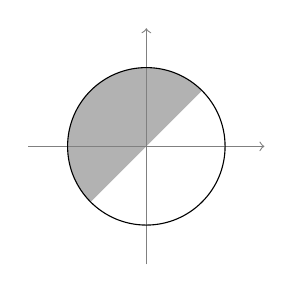
\begin{tikzpicture}[fill=black!30]
				\fill[rotate = 45] (0:0) -- (1, 0) arc (0:180:1) -- cycle;
				\draw[->][gray] (-1.5, 0) -- (1.5, 0);
				\draw[->][gray] (0, -1.5) -- (0, 1.5);
				\draw (0, 0) circle [radius = 1];
			\end{tikzpicture}
		\end{minipage}
		\begin{minipage}{10em}
			阴影部分 $ \sin\alpha > \cos\alpha $\\			
			空白部分 $ \sin\alpha < \cos\alpha $		
		\end{minipage}
	
		\subsection{判断 $\tan\alpha$ 与 $\cot\alpha$ 的大小}	
		\begin{minipage}{10em}
			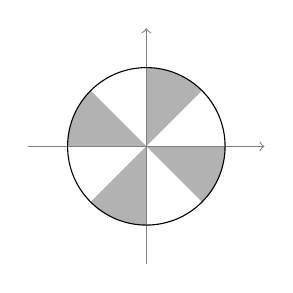
\begin{tikzpicture}[fill=black!30]
			\foreach \i in {0,...,3}
				\fill[rotate = 45 + \i * 90] (0:0) -- (1, 0) arc (0:45:1) -- cycle;
			\draw[->][gray] (-1.5, 0) -- (1.5, 0);
			\draw[->][gray] (0, -1.5) -- (0, 1.5);
			\draw (0, 0) circle [radius = 1];
			\end{tikzpicture}
		\end{minipage}
		\begin{minipage}{10em}
			阴影部分 $ \tan\alpha > \cot\alpha $\\
			空白部分 $ \tan\alpha < \cot\alpha $
		\end{minipage}
		
		\subsection{判断 $\tan\alpha$ 与 $\sin\alpha$ 大小}	
		\begin{minipage}{10em}
			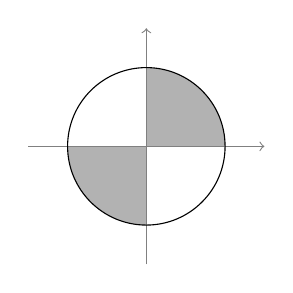
\begin{tikzpicture}[fill=black!30]
			\foreach \i in {0,...,1}
			\fill[rotate = \i * 180] (0:0) -- (1, 0) arc (0:90:1) -- cycle;
			\draw[->][gray] (-1.5, 0) -- (1.5, 0);
			\draw[->][gray] (0, -1.5) -- (0, 1.5);
			\draw (0, 0) circle [radius = 1];
			\end{tikzpicture}
		\end{minipage}
		\begin{minipage}{10em}
			阴影部分 $ \tan\alpha > \sin\alpha $\\
			空白部分 $ \tan\alpha < \sin\alpha $
		\end{minipage}
	
		\subsection{判断二倍角及半角象限}	
		\begin{minipage}{10em}
			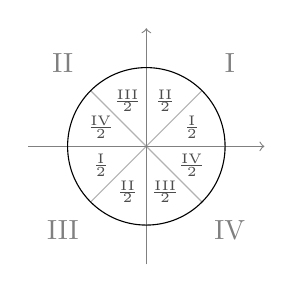
\begin{tikzpicture}[fill=black!30]
			\foreach \i in {0,...,3}
				\draw[black!30][rotate = 45 + \i * 90] (0:0) -- (0, 1);
			\draw[->][gray] (-1.5, 0) -- (1.5, 0);
			\draw[->][gray] (0, -1.5) -- (0, 1.5);
			\draw (0, 0) circle [radius = 1];
			\foreach \i in {1,...,4}
				\node[gray] at (-45 + 90 * \i:1.5) {\uppercase\expandafter{\romannumeral\i}};
	%		http://bbs.ctex.org/forum.php?mod=viewthread&tid=1534
			\foreach \i in {0,...,1}
				\foreach \j in {1,...,4}
					\node[font=\tiny][black!70] at (-22.5 + 180 * \i + 45 * \j :0.625) {$\rm \frac{\uppercase\expandafter{\romannumeral\j}}{2}$};
			\end{tikzpicture}
		\end{minipage}
		\begin{minipage}{10em}
			$\leftarrow$ \emph{看图}
		\end{minipage}
	
		\subsection{$t=\sin\alpha+\cos\alpha$ 取值}
		
		\begin{minipage}{10em}
			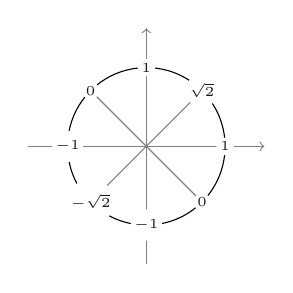
\begin{tikzpicture}[fill=black!30,
			label/.style={
				circle,
				font = \tiny,
				inner sep = 0.2mm,
				color = black!90,
	%			opacity=.95,
				fill=white}]
			\draw[->][gray] (-1.5, 0) -- (1.5, 0);
			\draw[->][gray] (0, -1.5) -- (0, 1.5);
			\draw[gray] (-135:1) -- (45:1);
			\draw[gray] (135:1) -- (-45:1);
			\draw (0, 0) circle [radius = 1];
			\node at (0:1) [label] {$1$};
			\node at (45:1) [label] {$\sqrt{2}$};
			\node at (90:1) [label] {$1$};
			\node at (135:1) [label] {$0$};
			\node at (180:1) [label] {$-1$};
			\node at (225:1) [label] {$-\sqrt2$};
			\node at (270:1) [label] {$-1$};
			\node at (315:1) [label] {$0$};
			%		http://bbs.ctex.org/forum.php?mod=viewthread&tid=1534
			\end{tikzpicture}
		\end{minipage}
		\begin{minipage}{10em}
		$\leftarrow$ \emph{看图}
		\end{minipage}
	
		\subsection{$t=\sin\alpha+\cos\alpha$ 取值}
		
		\begin{minipage}{10em}
			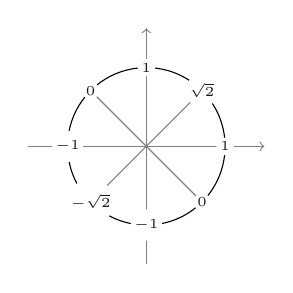
\begin{tikzpicture}[fill=black!30,
			label/.style={
				circle,
				font = \tiny,
				inner sep = 0.2mm,
				color = black!90,
				%			opacity=.95,
				fill=white}]
			\draw[->][gray] (-1.5, 0) -- (1.5, 0);
			\draw[->][gray] (0, -1.5) -- (0, 1.5);
			\draw[gray] (-135:1) -- (45:1);
			\draw[gray] (135:1) -- (-45:1);
			\draw (0, 0) circle [radius = 1];
			\node at (0:1) [label] {$1$};
			\node at (45:1) [label] {$\sqrt{2}$};
			\node at (90:1) [label] {$1$};
			\node at (135:1) [label] {$0$};
			\node at (180:1) [label] {$-1$};
			\node at (225:1) [label] {$-\sqrt2$};
			\node at (270:1) [label] {$-1$};
			\node at (315:1) [label] {$0$};
			%		http://bbs.ctex.org/forum.php?mod=viewthread&tid=1534
			\end{tikzpicture}
		\end{minipage}
		\begin{minipage}{10em}
			$\leftarrow$ \emph{看图}
		\end{minipage}
	
		
		\subsection{$t=\sin\alpha-\cos\alpha$ 取值}
		
		\begin{minipage}{10em}
			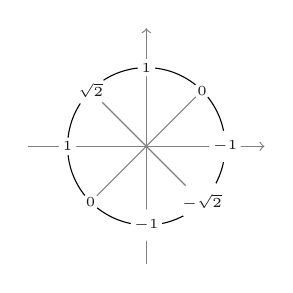
\begin{tikzpicture}[fill=black!30,
			label/.style={
				circle,
				font = \tiny,
				inner sep = 0.2mm,
				color = black!90,
				%			opacity=.95,
				fill=white}]
			\draw[->][gray] (-1.5, 0) -- (1.5, 0);
			\draw[->][gray] (0, -1.5) -- (0, 1.5);
			\draw[gray] (-135:1) -- (45:1);
			\draw[gray] (135:1) -- (-45:1);
			\draw (0, 0) circle [radius = 1];
			\node at (0:1) [label] {$-1$};
			\node at (45:1) [label] {$0$};
			\node at (90:1) [label] {$1$};
			\node at (135:1) [label] {$\sqrt2$};
			\node at (180:1) [label] {$1$};
			\node at (225:1) [label] {$0$};
			\node at (270:1) [label] {$-1$};
			\node at (315:1) [label] {$-\sqrt2$};
			%		http://bbs.ctex.org/forum.php?mod=viewthread&tid=1534
			\end{tikzpicture}
		\end{minipage}
		\begin{minipage}{10em}
			$\leftarrow$ \emph{看图啊你}
		\end{minipage}
	
		\subsection{六边形关系}
		\begin{center}
			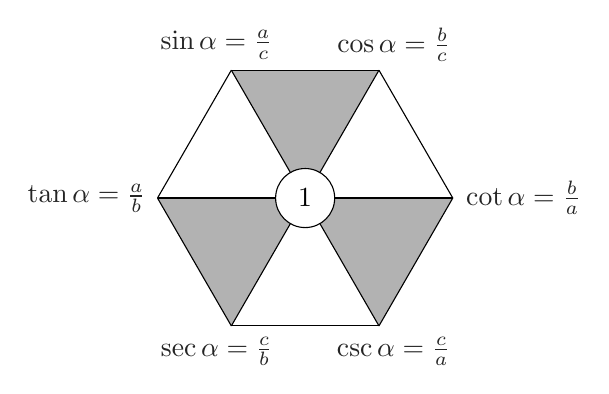
\begin{tikzpicture}[fill=black!30,
			scale=1.5,
			label/.style={
				rectangle,
				rounded corners = 1pt,
%				font = \small,
				inner sep = 0mm,
				color = black!90,
				opacity=.95,
				fill=white}]
			\foreach \i in {60, 180, 300}
				\fill (0, 0) -- (\i: 1.25) -- (60+\i: 1.25) -- cycle;
			\foreach \i in {0, 60,...,300}
			{
				\draw (\i: 1.25) -- (60+\i: 1.25);
				\draw (0, 0) -- (\i: 1.25);
			}
			\draw[fill=white] (0, 0) circle [radius = 0.25];
			\node at (0:1.85) [label] {$\cot\alpha = \frac b a$};
			\node at (60:1.5) [label] {$\cos\alpha = \frac b c$};
			\node at (120:1.5) [label] {$\sin\alpha = \frac a c$};
			\node at (180:1.85) [label] {$\tan\alpha = \frac a b$};
			\node at (240:1.5) [label] {$\sec\alpha = \frac c b$};
			\node at (300:1.5) [label] {$\csc\alpha = \frac c a$};
			\node at (0, 0) {1};
	%		http://bbs.ctex.org/forum.php?mod=viewthread&tid=1534
			\end{tikzpicture}
		\end{center}
		\begin{itemize}
			\item 对角线上两个三角函数乘积为 $1$
			\item 阴影三角形两上顶点的三角函数平方和等于下顶点的三角函数平方
			\item 任意顶点的三角函数等于相邻两顶点三角函数的乘积
		\end{itemize}
	}

	{
		\ctexset{section={afterskip = 0ex, fixskip = true}}
		\section{射影定理}
		\[ a = b \cos C + c \cos B \]
		\[ b = a \cos C + c \cos A \]
		\[ c = a \cos B + b \cos A \]
	}
	
	\end{multicols}

\end{document}
